\documentclass{JAC2003}

% As recommended here:
% http://www.ibic2013.org/IBIC2013/Participate/Paper-Preparation.html
\addtolength{\topmargin}{-18mm}

% This nonsense seems to be required to ensure that pdflatex processes this
% style correctly.
\ifx\pdfoutput\undefined
\else
\setlength{\paperwidth}{210mm}
\setlength{\paperheight}{296mm}
\setlength{\pdfpagewidth}{\paperwidth}
\setlength{\pdfpageheight}{\paperheight}
\fi


\usepackage{graphicx}       % Extended support for \includegraphics

\usepackage{array}          % Improved array support
\usepackage{booktabs}       % Publication quality tables

\usepackage{mathptmx}       % Mathematical PostScript fonts
\usepackage{amsmath}        % General mathematical symbols
\usepackage{textcomp}       % Extra symbols
\usepackage{mdwlist}

\usepackage{url}            % \url command for decent line breaks in urls
\usepackage{enumitem}       % For more control over list parameters.



\hyphenpenalty 4000 % Tone down hyphenation


\newcommand{\textsubscript}[1]{$_{\text{#1}}$}

\newcommand{\NCO}[1]{NCO\textsubscript{#1}}


\begin{document}
\title{CAPABILITY UPGRADE OF THE DIAMOND TRANSVERSE MULTIBUNCH FEEDBACK}

\author{%
    M.G.~Abbott, G.~Rehm, I.S.~Uzun,
    Diamond Light Source, Oxfordshire, UK}

\maketitle

\begin{abstract}

We describe an upgrade to the Transverse Multi-Bunch Feedback processor used
at Diamond for control of multibunch instabilities and measurement of betatron
tunes.  The new system will improve both feedback and diagnostic capabilities.
Bunch by bunch selectable control over feedback filters, gain and excitation
will allow finer control over feedback, allowing for example the single bunch
in a hybrid or camshaft fill pattern to be controlled independently from the
bunch train.  It will also be possible to excite all bunches at a single
frequency while simultaneously sweeping the excitation for tune measurement of
a few selected bunches.  The single frequency excitation can be used for bunch
cleaning or continuous measurement of the beta-function.  A simple
programmable event sequencer will provide support for up to 8 steps of
programmable sweeps and changes to feedback and excitation, allowing a variety
of complex and precisely timed beam characterisation experiments including
grow-damp measurements in unstable conditions.

\end{abstract}


\section{Introduction}

At Diamond we stabilise transverse oscillations of the bunches with two FPGA
based Transverse Multi-Bunch Feedback processors, one operating horizontally,
one vertically.  Each processor is a Libera Bunch-by-Bunch from Instrumentation
Technologies \cite{libera}, packaged as a 1U unit containing 4 14-bit ADCs
running at 125\,MHz, a Virtex-II Pro FPGA clocked at 125\,MHz, a 14-bit DAC
running at 500\,MHz, and an embedded Single Board Computer (SBC) ARM
microprocessor running Linux to provide the control system.

The system was delivered as a basic development platform with basic interfacing
software on the Linux board and a layer of FPGA code for interfacing to the
external signals and the processor board.  The initial implementation of the
Transverse Multi-Bunch Feedback (TMBF) processor was done by Isa Uzun and was
based on work at the ESRF \cite{esrf}.  The Diamond implementation consists of
FPGA code together with an EPICS driver running on the embedded processor board
\cite{early-tmbf}.

The first version of the TMBF system has now been running at Diamond since 2007
and provides good support for beam stabilisation through transverse feedback and
tune measurement, but limited support for more advanced experiments.

The developments described in this paper, still very much work in progress,
provide support for more detailed measurements, finer control, and more complex
experiments.  In particular, the following major functionality is added in this
update:

\begin{itemize}
\item
    Separate feedback parameters for individual bunches.  For example, we can
now use one feedback filter for the hybrid bunch and a different filter for the
rest of the fill.
\item
    Concurrent tune measurements on up to four different bunches.
\item
    Program sequencing, allowing a sequence of different control parameters to
be applied to the beam at the same time as data capture.
\item
    Output gain compensation to compensate for high frequency roll-off.
\end{itemize}

A key concept here is the \emph{bunch number}: in the train of 936 bunches in
the storage ring, each bunch is assigned its own sequence number, and processing
parameters are configured separately for each bunch.  The location of
\emph{bunch zero} is defined through an external trigger.


\section{Motivation}

Diamond has been using a transverse multibunch feedback (TMBF) since 2007
\cite{early-tmbf, performance}.  This system, while using the Libera
Bunch-by-Bunch hardware utilises an in-house developed FPGA code and EPICS
interface.  The firmware and software have continued to develop and include
functionality beyond the pure feedback action required for suppression of
multibunch instabilities.  Namely, a Numerically Controlled Oscillator (NCO)
with a programmable sweep function together with a numerical I/Q mixer and
accumulator have enabled continuous measurement of the betatron tune oscillation
frequency \cite{status} with minimal disturbance to the beam.

However, new operational requirements demand further functionality so a major
upgrade of the FPGA and supporting EPICS interface has been implemented to
enhance the capabilities of the existing system.  These requirements can be
classified as follows:


\subsection{Timed Sequence Experiments}

Some experiments require several states of the system to be processed in a
tightly timed sequence.  One example is ``grow-damp'' experiments where a
certain mode of oscillation is first grown (either forced by the NCO or
naturally due to an instability), and subsequently damping is observed (either
synchrotron radiation damping or forced damping using the feedback).  In the old
implementation, only a ``permanent'' and a ``temporary'' state were available,
allowing for ``feedback-off-feedback'' or ``off-NCO-off''.  However, there are
interesting operational conditions near the instability threshold which cannot
be adequately investigated using just one temporary state.  Also, observing the
natural growth of an instability is highly unpredictable unless the growth rate
is already very high.  In this case the desired sequence would be
``feedback-NCO-off-feedback'' to drive a potentially unstable mode first, then
observe whether it is damping naturally, then switch back to feedback.   Another
sequence of steps would be repeated measurements of the tune using a fast sweep
(while exciting one or many bunches), followed by a slow sweep of a narrower
range with strong excitation of just a few bunches which are supposed to be
cleared from the storage ring to improve the purity of the fill pattern.


\subsection{Differing Actions per Bunch}

Some experiments require different actions on different bunches.  With the old
implementation this was partially possible, allowing for a selection of feedback
or NCO excitation on a bunch by bunch basis.  However, all bunches had to see
the same NCO excitation.  We have demonstrated an approach for measuring the
beta function of the storage ring during user mode operation \cite{measurement},
which requires continuous excitation of all bunches at the betatron frequency
which is then detected by all electron beam position monitors.  In order to make
this compatible with continuous measurement of the betatron tune, the TMBF must
be able to feedback on all bunches except one and simultaneously excite these
with a fixed frequency NCO, while at the same time sweeping an excitation for
one bunch to measure the tune.  The new implementation allows bunch-by-bunch
selection of any combination of feedback, \NCO1 (fixed frequency) or \NCO2
(swept frequency).


\subsection{Capturing High Volumes of Data}

Experiments which require large amounts or frequent collection of
bunch-by-bunch data: in the previous implementation access to the large
bunch-by-bunch data buffer  was not possible through the EPICS interface and
instead required command line access, which was cumbersome and unreliable.
Collection of data from frequently occurring events, like from the disturbance
due to the injection kickers during each top-up was not possible.  The new
implementation has access to this buffer fully integrated into the EPICS
interface.  Access to large amounts of bunch-by-bunch data will facilitate a
continuously updating display of an instability analysis mode by mode.


\subsection{Improving System Impulse Response}

Improving the impulse response of the system: measurements of the impulse or
frequency response of the TMBF system have shown cross talk between adjacent
bunches, which leads to a low pass behaviour in the frequency response.  We
concluded that this can be mitigated to some degree by implementing a digital
``pre-emphasis'' filter acting on the samples just in front of the final digital
output to the DAC.


\begin{figure*}[!ht]
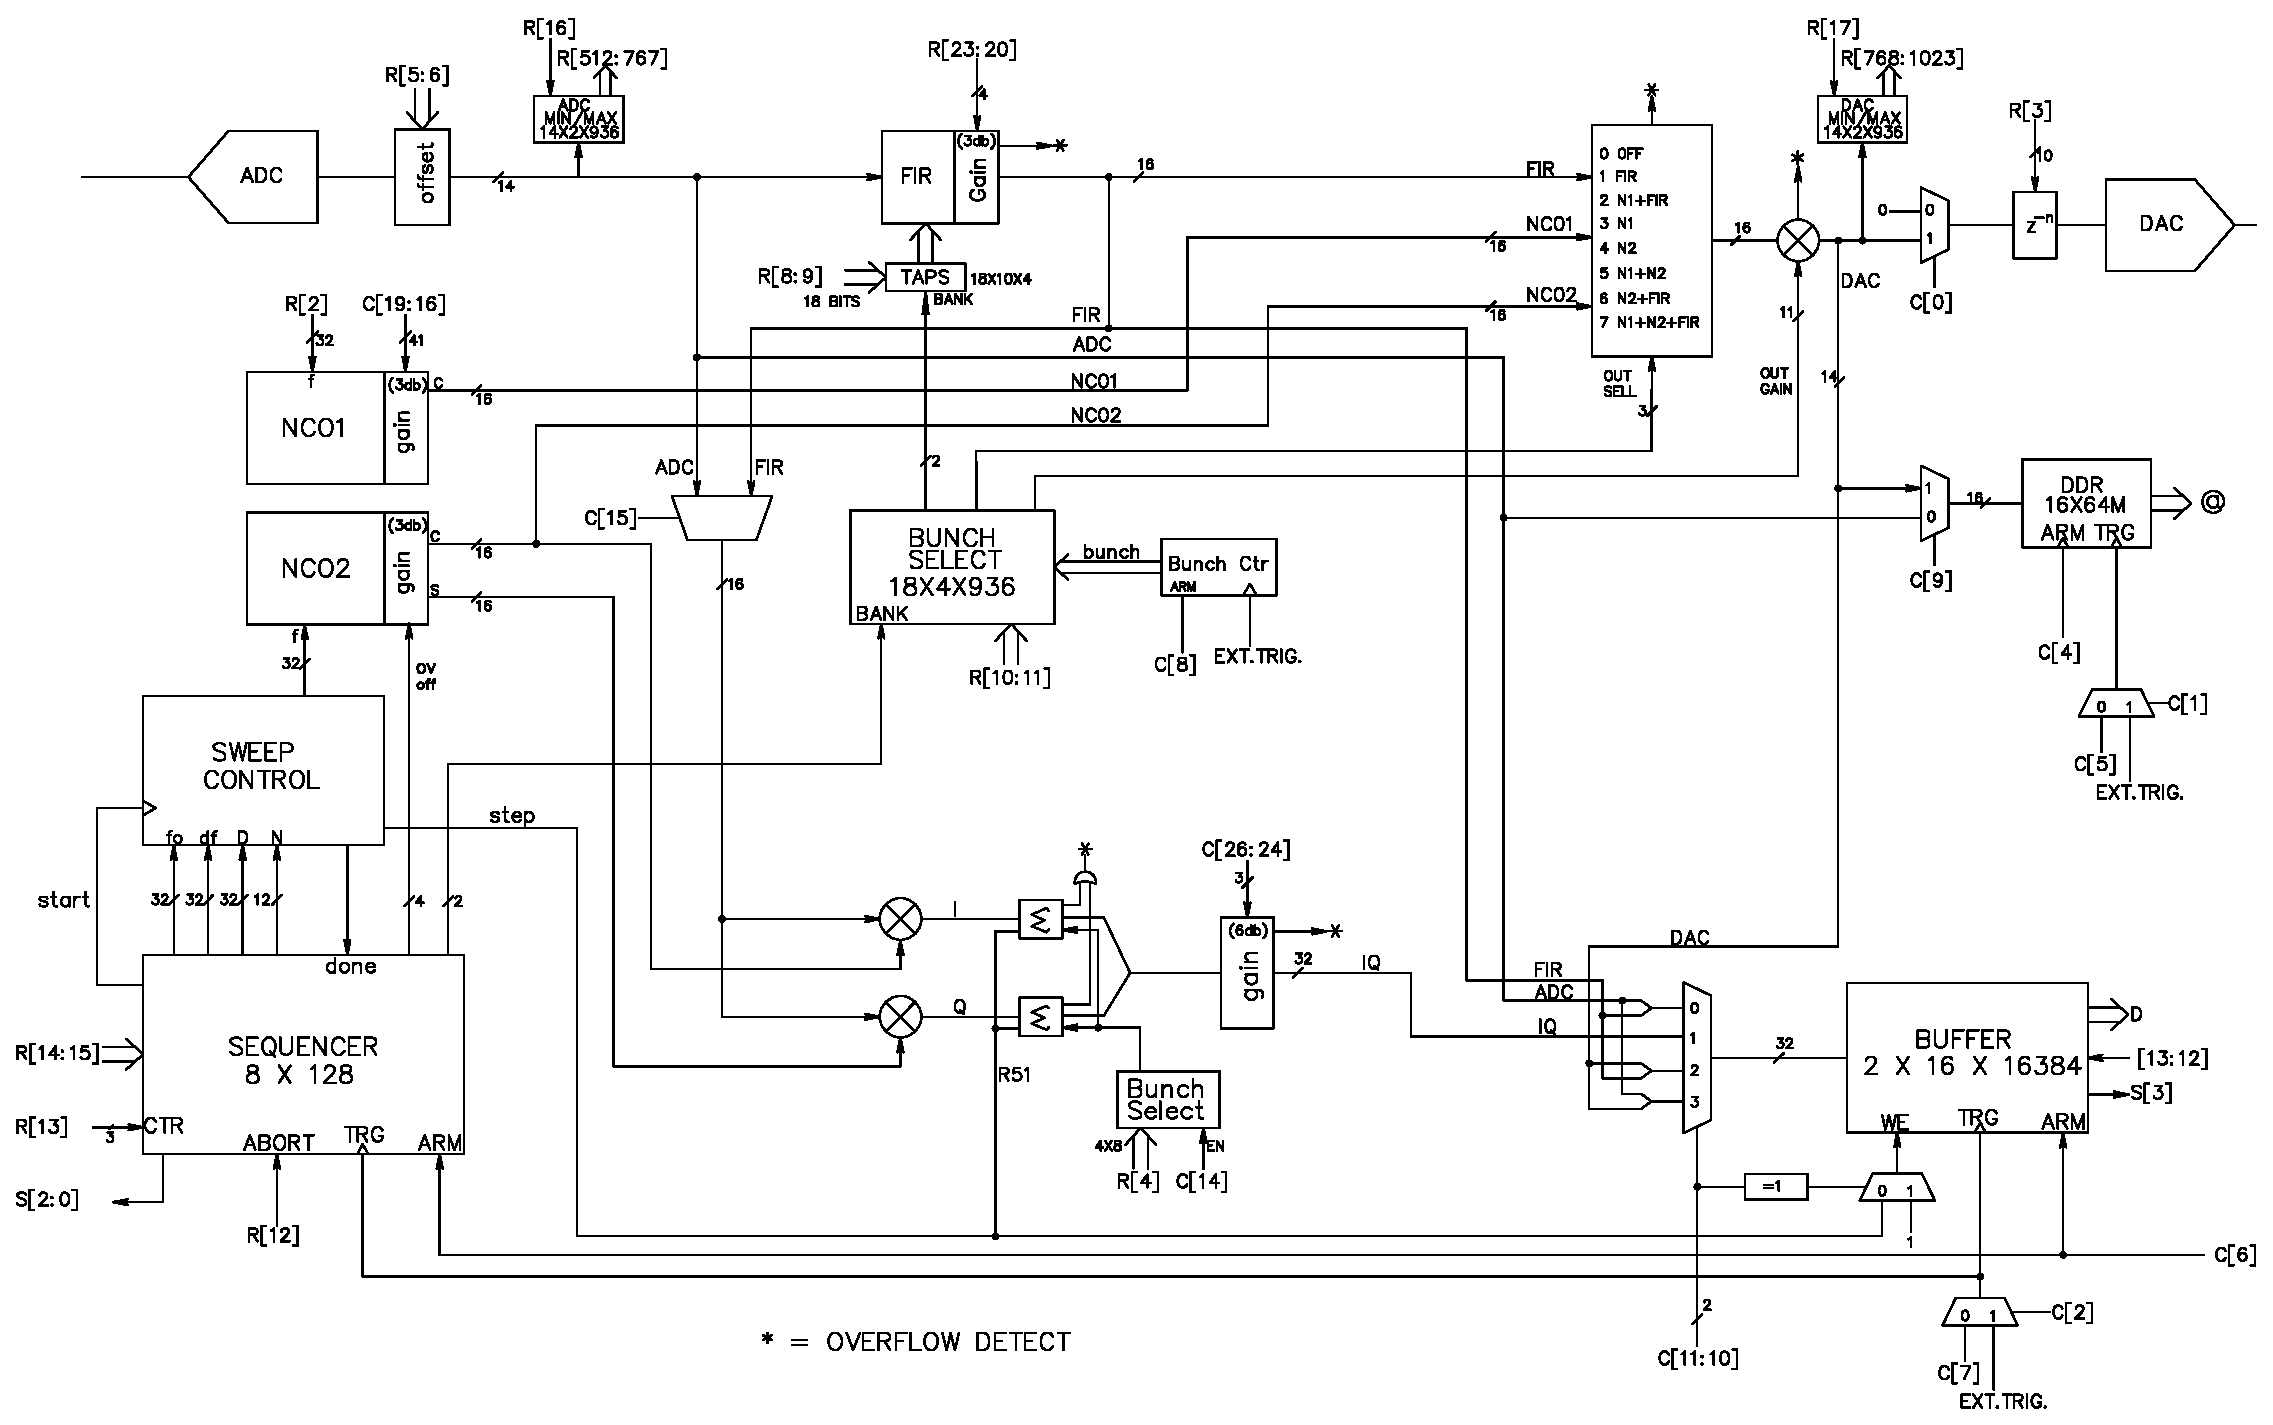
\includegraphics[width=\linewidth]{WEPC10f1}
\caption{Approximate Internal FPGA architecture of TMBF Processor}
\label{fpga:architecture}
\end{figure*}



\section{Implementation}

The implementation of the TMBF is a mixture of FPGA code (written in System
Verilog) and the EPICS driver (written in C).  The structure of the FGPA
implementation is shown in Fig \ref{fpga:architecture}.  The development
strategy has been to ensure that high speed and intensive processing is
performed in the FPGA but to off-load as much complexity as possible into the
internals of the EPICS driver.  For instance, there are numerous places within
the TMFB processing chain where the bunch number affects processing: this is
measured and compensated in software, rather than creating long delay lines in
the FPGA.

One interesting complication in the FPGA implementation arises from a speed
mismatch: the machine RF frequency is 500\,MHz with bunches separated by 2\,ns,
but the ADCs and core FPGA processing can only running at 125\,MHz.  This is
resolved by running four concurrent channels of processing inside the FPGA.
Mostly this is hidden and demultiplexed in software, but we take advantage of
this to implement simultaneous bunch detection on four separate bunches.

The FPGA provides the following elements:
\begin{itemize}
\item Core processing chain from ADC to DAC.
\item Data capture from FPGA to EPICS clients.
\item Frequency generator and detector, the basis of tune measurement.
\item Sequencer and bunch configuration selection.
\end{itemize}

\subsection{Core Processing Chain}

This is the core feedback chain consisting of data capture, filtering,
excitation injection and output pre-emphasis.  This chain comprises the
following stages:

\begin{description}

\item[Input.] Interfaces to the ADC and performs offset compensation for small
ADC voltage offsets between the four ADCs.

\item[Filtering.] Filters with up to ten taps can be applied to each bunch in
turn.  Each bunch can have its own filter, from a choice of four programmable
filters.  The result of filtering is scaled and checked for overflow: any
overflow is reported through the EPICS interface.

\item[Output Selection.] For each bunch the generated output signal can be
selected as a sum of up to three sources: the filtered input, or one or both
NCOs.  Also, each bunch has its own scaling applied at this stage.  Again
overflow is checked for and detected.

\item[Output.] The output data stream is now filtered with a three tap filter
for output compensation and delayed by a programmable delay of up to a full
machine turn: this is used to compensate for external delays to ensure that each
bunch is processed separately.  Again, numeric overflow is checked and reported.

\end{description}


\subsection{Data Capture}

\subsubsection{Min/Max ADC and DAC.}

For both the incoming bunch measurements (after offset compensation) and the
outgoing drive signal the FPGA internally records the minimum and maximum value
read and written for each bunch.  These measurements are read and reset by the
control system and used to generate EPICS waveforms to provide a very helpful
overview of bunch movements and system activity.

\subsubsection{Long Buffer.}

A very long buffer can capture up to 64\,M samples, or around 100\,ms, of ADC,
FIR or DAC data.  This acquisition can be triggered by software or from an
external trigger.

The EPICS interface provides an overview of the captured data and a defined
mechanism for reading out the entire waveform.  Data can be read out at around
1,000,000 samples per second, mainly limited by control processor capacity.

\subsubsection{Short Buffer.}

A short double width buffer can capture up to 16,384 samples of two out of three
of ADC, FIR or DAC data, or can be used to capture IQ detector data when a
frequency sweep is being generated.

The I/Q data is processed in the control system to generate tune response data
as EPICS waveforms and a tune value is extracted.


\subsection{Frequency Generator and Detector}

\NCO1 has a fixed programmable frequency which can be added into selected
bunches for fixed excitation.  \NCO2 is controlled by the sequencer to generate
a swept frequency which can also be added to selected bunches.

The swept NCO dwells for a programmable number of turns at each frequency and
during this dwell an IQ detector mixes the NCO output with either the ADC or FIR
signal to generate a response measurement at this frequency.  The detector can
either observe all bunches or a single selected bunch.

The resulting IQ value generated by the detector is then written to the short
buffer, and so after performing a complete sweep the response waveform can read
out and is used to compute the tune response.


\subsection{Sequencer and Bunch Selector}

At the heart of the advanced experimental functionality of the TMBF is the
sequencer and bunch selection array.  The sequencer has up to seven states (plus
a quiescent state for normal operation) which can be programmed and then
triggered.  When triggered the sequencer will progress through the selected
states, changing the operation of the TMBF accordingly, and capturing IQ
detector data as appropriate.

Each state of the sequencer defines the following controls:

\begin{itemize}
\item Start frequency and frequency step for \NCO2.
\item How many turns to excite at the selected frequency, or ``dwell time''.
\item Total number of frequency steps: so total duration is number of steps
multiplied by dwell time.
\item Excitation gain.
\item Bunch configuration selection.
\end{itemize}

The bunch configuration selection provides the flexibility of this system: up to
four different bunch configurations can be programmed, and each sequencer state
can select a different configuration.  For each of the four available bunch
configurations the following parameters are defined for each bunch:

\begin{itemize}
\item Filter: one of four different programmable filters can be selected for
each bunch.
\item Output selection: any or none of the FIR, \NCO1 or \NCO2 outputs can be
combined and accumulated per bunch.
\item Output gain: each bunch can be driven with separately selected intensity.
\end{itemize}

For example, in one configuration feedback can be enabled on one bunch, active
excitation can be driven onto its neighbours, and finally the rest of the train
can be left undisturbed.



\begin{figure}[h]
\centering
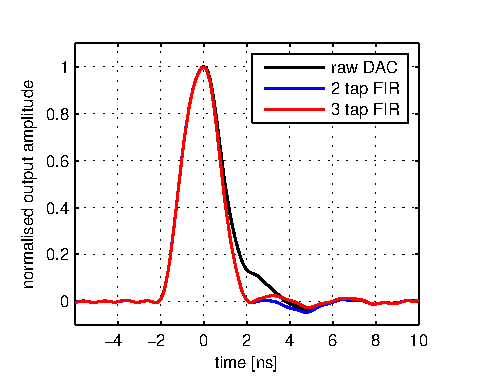
\includegraphics{WEPC10f2}
\caption{Effect of output pre-compensation on DAC output}
\label{precomp}
\end{figure}


\section{Output Pre-Compensation}

One of the goals of the TMBF is to operate on each bunch independently of its
neighbours.  There is enough bandwidth in the system for this to be a sensible
goal, but there is some spill-over between adjacent bunches in the DAC output.
Much of this effect can be cancelled out by a simple three tap pre-compensation
filter on the output.

Fig \ref{precomp} shows three oscilloscope traces measured on a high bandwidth
scope showing the raw DAC output and the cancelling effect of precompensation.
Note that with all three taps it is possible to cancel out most interference
between bunches.



\section{Conclusions}

At the time of writing this is still very much work in progress.  Results from
live operation on the Diamond synchrotron should be available towards the end of
the year.



\begin{thebibliography}{9}

\bibitem{libera}
Instrumentation Technologies, \emph{Libera Bunch-by-Bunch},
\url{http://www.i-tech.si}.

\bibitem{esrf}
E.~Plouviez, P.~Arnoux, F.~Epaud, J.~Jacob, J.M.~Koch, N.~Michel, G.A.~Naylor,
J.\mbox{-}L.~Revol, V.~Serriere, D.~Vial, \emph{Broadband Bunch by Bunch
Feedback for the ESRF using a Single High Resolution and Fast Sampling FPGA
DSP}, EPAC~2006.

\bibitem{early-tmbf}
A.F.D.~Morgan, G.~Rehm, I.~Uzun, \emph{First Tests of the Transverse Multibunch
Feedback at Diamond}, DIPAC~2007

\bibitem{performance}
A.F.D.~Morgan, G.~Rehm, I.~Uzun, \emph{Performance and Features of the Diamond
TMBF System}, EPAC~2008.

\bibitem{status}
I.~Uzun, M.G.~Abbott, M.T.~Heron, A.F.D.~Morgan, G.~Rehm, \emph{Operational
Status of theTransverse Multibunch Feedback System at Diamond}, ICALEPCS~2011.

\bibitem{measurement}
G.~Rehm, M.G.~Abbott, A.F.D.~Morgan, J.~Rowland, I.~Uzun, \emph{Measurement of
Lattice Parameters Without Visible Disturbance to User Beam at Diamond Light
Source}, BIW~2010.


\end{thebibliography}


\end{document}
